\subsection{Small-scale evaluations}
\label{sec:small-scale}

\begin{figure}[htbp]
  \centering
  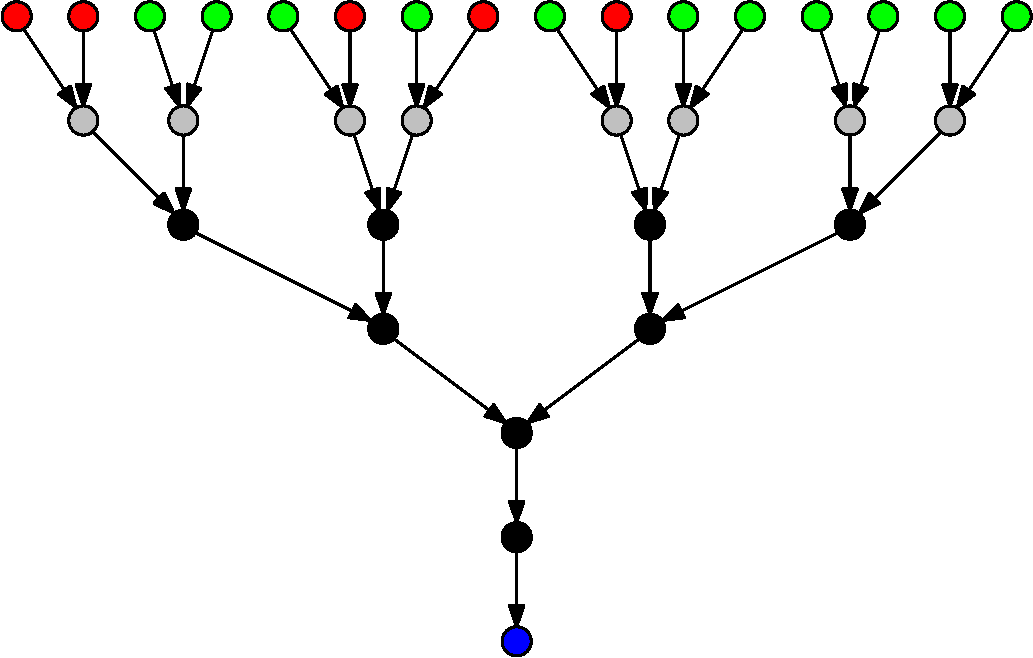
\includegraphics[scale=0.3]{topo-tree-evil-5-good-0-producer-gw}
  \caption{Small-scale topology (one of the runs with 30\% of attackers, all links are 10Mbps with randomized delay 1-10ms)}
  \label{fig:small-scale-topo}
\end{figure}


\begin{figure}[htbp]
  \centering
  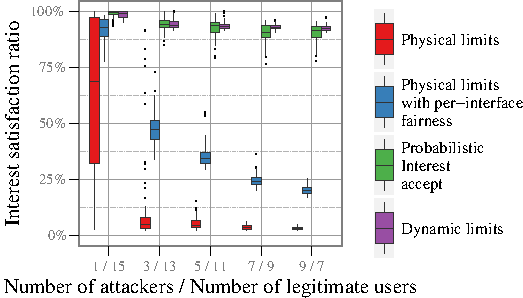
\includegraphics[scale=1]{tree-topo-var-evils-max-consumers-30mins/tree-good-0-producer-gw-avg-1-min}
  \caption{Average consumer Interest satisfaction ratios (first minute)}
  \label{fig:small-scale-topo 1}
\end{figure}


\begin{figure}[htbp]
  \centering
  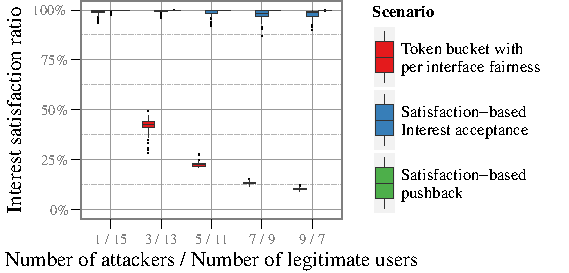
\includegraphics[scale=1]{tree-topo-var-evils-max-consumers-30mins/tree-good-0-producer-gw-avg-1-min-after-1-min}
  \caption{Average consumer Interest satisfaction ratios (second minute)}
  \label{fig:small-scale-topo 2}
\end{figure}

\begin{figure}[htbp]
  \centering
  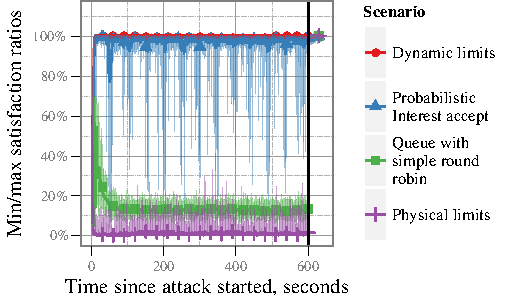
\includegraphics[scale=1]{tree-topo-var-evils-max-consumers-30mins/tree-good-0-producer-gw-dynamics-40}
  \caption{Satisfaction ratio dynamics during the attack (7 attackers / 9 legitimate)}
  \label{fig:small-scale-topo 3}
\end{figure}


%%% Local Variables: 
%%% mode: latex
%%% TeX-master: "paper"
%%% End: 
